% !TeX encoding = UTF-8
% !TeX program = latexmk
% !TeX root = ../latex-talk.tex

\section{学位论文排版}
\subsection{\ThuThesis 清华大学学位论文模板}

\begin{frame}{\ThuThesis}
  \framesubtitle{清华大学学位论文 \LaTeX{} 模板}
  \begin{itemize}
  \item 最早由王磊于 2004年4月发布,2005 年薛瑞尼接手维护,2018年起李泽平为主力开发者,2020年起由TUNA维护
  \item 最新正式版:\ThuThesisVersion\ (\ThuThesisDate)
  \item 全面支持最新的本科、研究生\footnote{更新到\ThuThesisGuideVersion{}发布的《清华大学研究生学位论文写作指南》,并支持若干院系的特殊要求}、博士后论文/报告格式,获研究生院官方推荐 \link{https://info2021.tsinghua.edu.cn/f/info/xxfb_fg/xnzx/template/detail?xxid=fa880bdf60102a29fbe3c31f36b76c7e}
  \end{itemize}
  \begin{figure}[htbp]
    \centering
    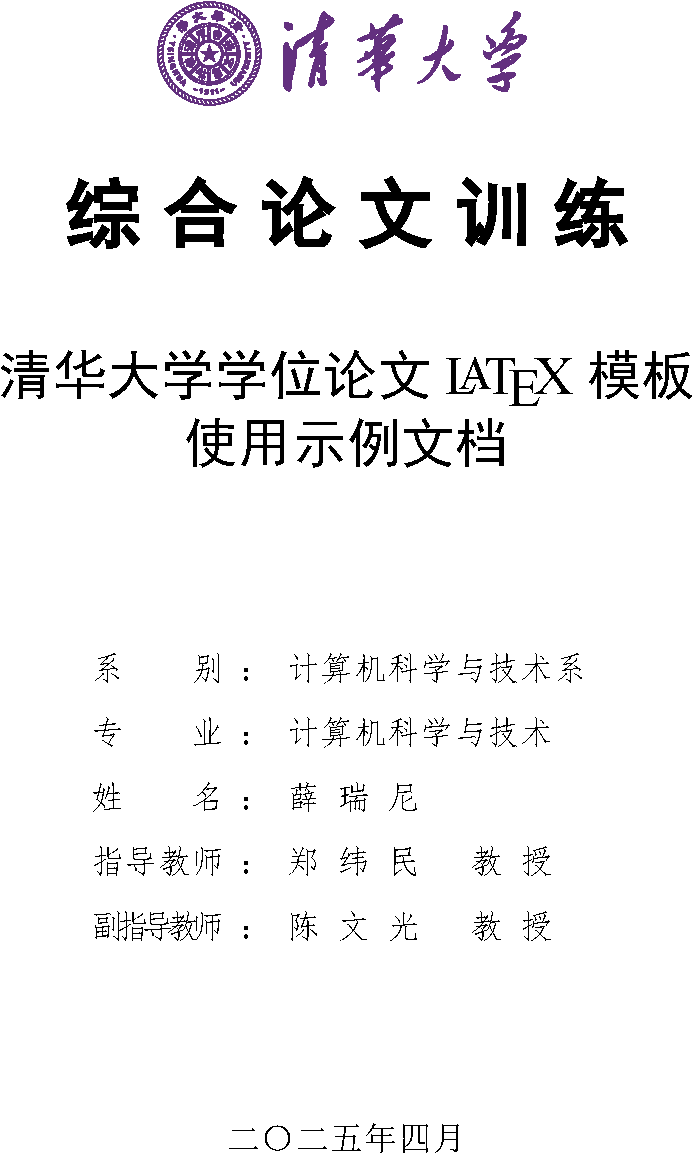
\includegraphics[height=.4\textheight]{cover-bachelor-crop.pdf}\hfill
    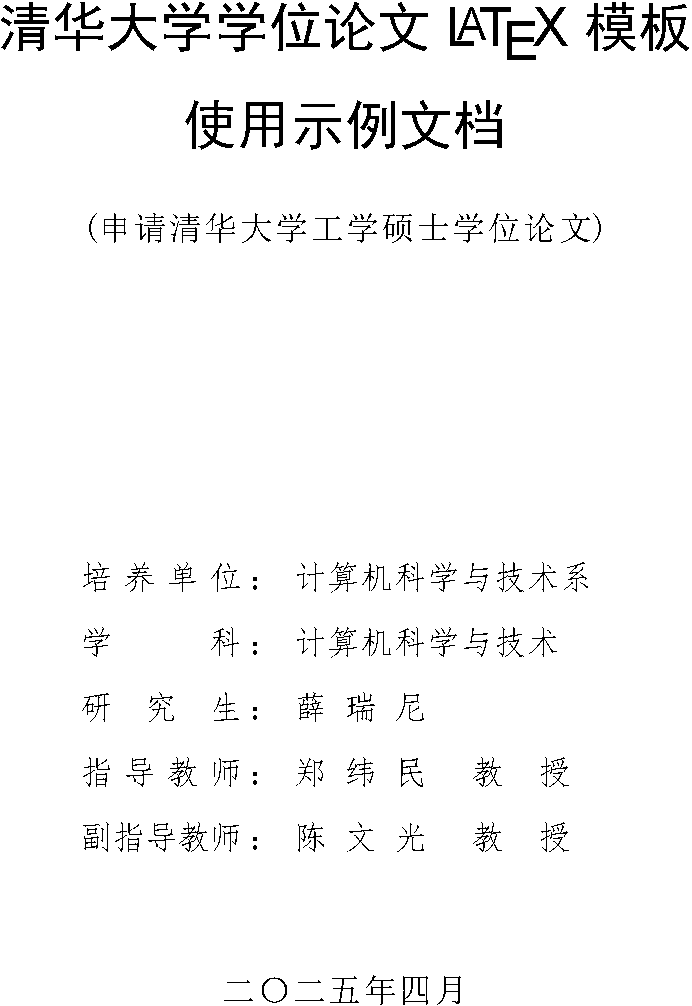
\includegraphics[height=.4\textheight]{cover-master-crop.pdf}\hfill
    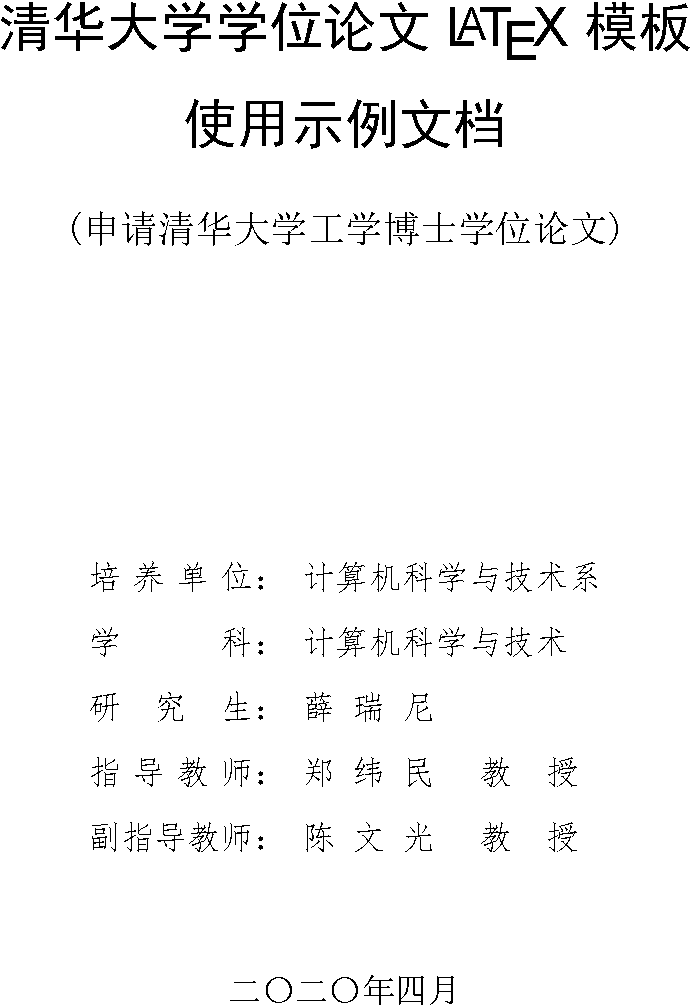
\includegraphics[height=.4\textheight]{cover-doctor-crop.pdf}\hfill
    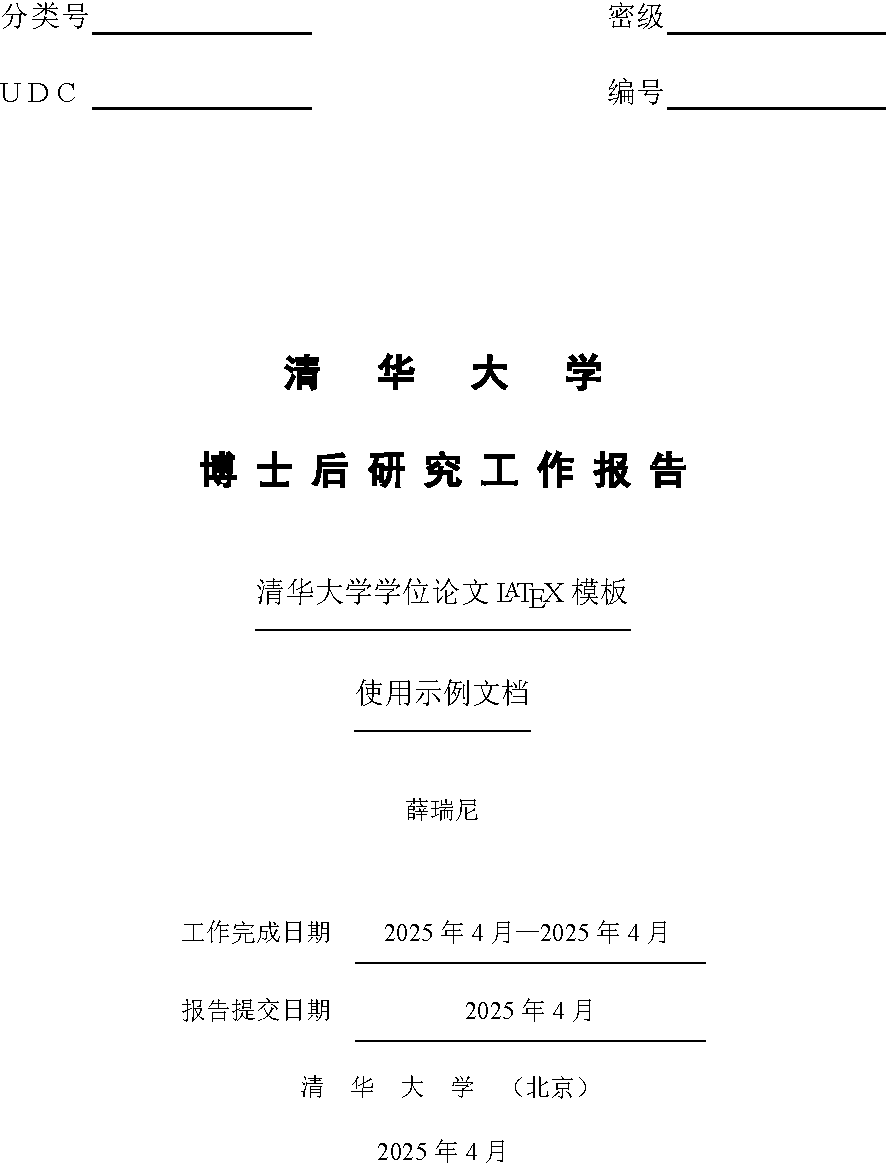
\includegraphics[height=.4\textheight]{cover-postdoc-crop.pdf}
  \end{figure}
\end{frame}

\begin{frame}[fragile]{手动安装\ThuThesis{}}
      \begin{columns}
        \begin{column}{.75\textwidth}
  \begin{itemize}
    \item 下载最新正式版(推荐)
      \begin{itemize}
        \item CTAN 官方 \link{http://mirrors.ctan.org/macros/latex/contrib/thuthesis.zip}(发行版可使用自带更新机制)
        \item GitHub Releases \link{\ThuThesisLink/releases} 或 TUNA 镜像 \link{https://mirrors.tuna.tsinghua.edu.cn/github-release/\ThuThesisRepo/}
      \end{itemize}
    \item 从 CI 下载最新开发版(高级 / 想尝鲜 / 着急的用户)
      \begin{itemize}
        \item \url{\ThuThesisLink}
        \item 点击 master 分支的小绿勾——点击“build”一项旁边的“Details”链接进入 CI 详情
        \item 点击左侧边栏“Summary”——滚动页面到最底下,从“Artifacts”中选择 |build-snapshot-release| 下载
        \item 解压下载的 ZIP 文件,得到 |dist/thuthesis-v*.zip|
      \end{itemize}
  \end{itemize}
        \end{column}
        \begin{column}{.25\textwidth}
          \begin{figure}[htbp]
            \centering
            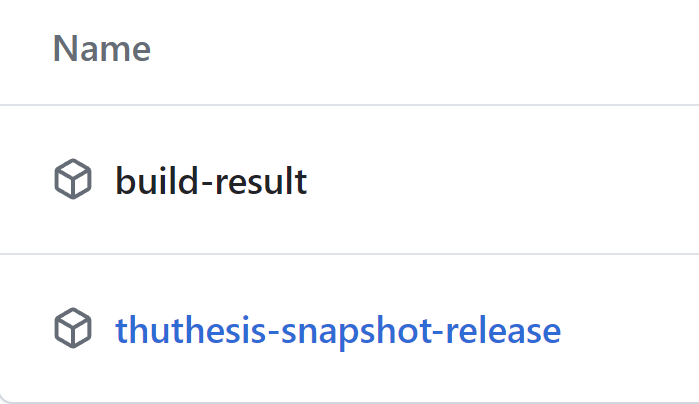
\includegraphics[width=.95\textwidth]{thuthesis-download.png}
          \end{figure}
        \end{column}
      \end{columns}
  \begin{itemize}
    \item 编译与安装
      \begin{itemize}
        \item 解压缩 |thuthesis-v*.zip| 后\textbf{先看文档} |README.md|
        \item 模板文档类:|thuthesis.cls| 已经编译好,无需额外操作
        \item 论文示例:|make thesis| 编译 |thuthesis-example.tex| $\Rightarrow$
        |thuthesis-example.pdf|
        \item 用户手册:|make doc| 编译 |thuthesis.dtx| $\Rightarrow$
          |thuthesis.pdf|
        \item 更多用法可参考附带的 |Makefile|
      \end{itemize}
  \end{itemize}
\end{frame}

\begin{frame}[fragile]{模板选项}
\begin{description}
\item[degree] 指定学位类型(本科/硕士/博士/博后)
  \begin{lstlisting}[basicstyle=\ttfamily]
\documentclass[degree=bachelor]{thuthesis}
  \end{lstlisting}
\item[degree-type] 指定学位选项(专硕/学硕格式不同)
  \begin{lstlisting}[basicstyle=\ttfamily]
\documentclass[degree=master,degree-type=professional]{thuthesis}
  \end{lstlisting}
\item[fontset] 指定字体(推荐使用 |windows|,详见模板文档说明)
  \begin{lstlisting}[basicstyle=\ttfamily]
\documentclass[degree=doctor,fontset=windows]{thuthesis}
  \end{lstlisting}
\end{description}
\end{frame}

\begin{frame}[fragile]{封面}
  使用 |\thusetup| 命令指定论文各类选项:
  \begin{table}[h]
    \centering
\footnotesize
  \begin{tabular}{lll} \toprule
    命令作用 & 中文对应选项 & 英文对应选项 \\ \midrule
  论文标题 & |title| & |title*| \\
  作者姓名&  |author| &|author*|\\
  申请学位类型 & |degree-category|&|degree-category*|\\
  院系名称 & |department| & |department*|\\
  学科名称 & |discipline| & |discipline*|\\
  专业领域 & |professional-field| & |professional-field*|\\
  导师 & |supervisor| & |supervisor*|\\
  副导师 & |associate-supervisor| & |associate-supervisor*|\\
  联合导师 & |joint-supervisor| & |joint-supervisor*|\\
  日期 & \multicolumn{2}{c}{\texttt{date}}\\
  密级 & \multicolumn{2}{c}{\texttt{secret-year, secret-level}}\\
  语言(环境名称等) & \multicolumn{2}{c}{\texttt{language}} \\ 
  博后专用 & \multicolumn{2}{c}{\texttt{clc, udc, id, ...}} \\ \bottomrule
  \end{tabular}
  \end{table}
\end{frame}

\begin{frame}[fragile]{数学}
  \begin{itemize}
    \item 公式示例:\nolinkurl{data/chap01.tex}
    \item \ThuThesis{} 定义了常用的数学环境(需要手工引入 |amsthm| 宏包):
      \begin{table}[h]
        \centering
        \footnotesize
\begin{tabular}{*{7}{l}}\toprule
  axiom & theorem & definition & proposition & lemma & conjecture &\\
  公理 & 定理 & 定义 & 命题 & 引理 & 猜想 &\\\midrule
  proof & corollary & example & exercise & assumption & remark & problem \\
  证明 & 推论 & 例子& 练习 & 假设 & 注释 & 问题\\\bottomrule
\end{tabular}
      \end{table}
      \item \ThuThesis{} 使用 \pkg{unicode-math} 进行数学输入(\ref{frame:unicode-math} 页),注意与传统方式的区别
  \end{itemize}
\end{frame}

\begin{frame}[fragile]{参考文献}
  \begin{itemize}
    \item 使用 \BibTeX 和 \pkg{natbib} 宏包
      \begin{itemize}
        \item 本科生文献翻译/阅读报告的参考文献与正文独立
        \item 推荐使用 |latexmk| 编译以保证参考文献生成正确
      \end{itemize}
    \item 模板支持两种引用方式:
      \begin{itemize}
        \item 顺序编码制(默认),其中包含两种模式:
        \begin{itemize}
          \item 上标模式:如“在许多文献\textsuperscript{[12-13]}中……”
          \begin{lstlisting}[basicstyle=\ttfamily]
    \cite{key12, key13}
          \end{lstlisting}
        \item 正文模式:如“文献~[14] 证明了……”
          \begin{lstlisting}[basicstyle=\ttfamily]
    \inlinecite{key14}
          \end{lstlisting}
        \end{itemize}
        \item 著者-出版年制,包括两种引用模式(\cmd{citep}, \cmd{citet})
      \end{itemize}
    \end{itemize}
\end{frame}

% \begin{frame}{作图}
%   \begin{columns}[c]
%     \begin{column}{.5\textwidth}
%   \begin{itemize}
%   \item 矢量图 eps, ps, pdf
%     \begin{itemize}
%     \item \MP, pstricks, pgf $\ldots$
%     \item Xfig, Dia, \alert{Visio}, \alert{Inkscape} $\ldots$
%     \item Matlab / Excel 等保存为 pdf
%     \end{itemize}
%   \item 标量图 png, jpg, tiff $\ldots$
%     \begin{itemize}
%       \item 提高清晰度,避免发虚
%     \end{itemize}
%   \item 转化
%     \begin{itemize}
%     \item 虚拟打印机
%     \item ImageMagick
%     \item epstopdf
%     \item pdfcrop
%     \end{itemize}
%   \end{itemize}
%     \end{column}
%     \begin{column}{.4\textwidth}
% \begin{figure}[h]
%   \centering
% \includegraphics[height=.3\textheight]{shapepar.pdf}\\\vspace{1cm}
% 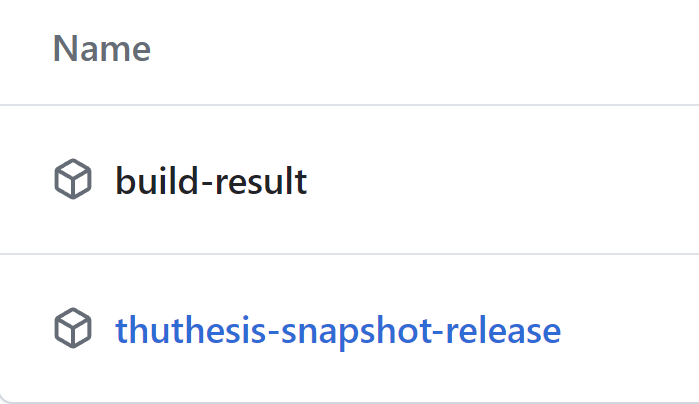
\includegraphics[height=.3\textheight]{thuthesis-download.png}
% \end{figure}
%     \end{column}
%   \end{columns}
% \end{frame}

\begin{frame}[fragile]{\ThuThesis 问题}
    \begin{itemize}
      \item 常见问题
        \begin{itemize}
          \item 参考文献列表出错、缺少字体、无法编译、格式不对……:先\textbf{更新到最新版本}试试
          \item 认真阅读文档 |thuthesis.pdf| 和使用示例 |thuthesis-example.pdf|
          \item 查看 FAQ \link{\ThuThesisLink/wiki/FAQ}
        \end{itemize}
      \item 主动提问
        \begin{itemize}
          \item GitHub Discussions 提问 \link{\ThuThesisLink/discussions}
          \item GitHub Issues 提交 bug \link{\ThuThesisLink/issues}
          % \item \TeX @newsmth 查找或发文
          % \item \ThuThesis{} Google Group 发问 \link{http://groups.google.com/group/thuthesis}
        \end{itemize}
    \end{itemize}
\end{frame}



%%% vim: set sw=2 isk+=\: et tw=80 cc=+1 formatoptions+=mM:
